\index{OpenQuake-engine!risk}

The seismic risk results are being calculated using the OpenQuake risk library
(oq-risklib), an open-source suite of tools for seismic risk assessment and
loss estimation. This library is written in the Python programming language
and available in the form of a ``developers'' release, that can be executed
through a command line interface. The code of the library can be found on a
public repository at GitHub at the following address
\href{http://github.com/gem/oq-risklib}{http://github.com/gem/oq-risklib}.

The risk component of the OpenQuake-engine can compute both scenario-based and
probabilistic seismic damage and risk using various approaches. The following
types of analysis are currently supported:

\begin{itemize}

    \item \textit{Scenario Damage Assessment}, allowing the calculation of
	damage distribution statistics for a portfolio of buildings from a single
	earthquake rupture scenario taking into account aleatory and epistemic
	ground-motion variability.

	\item \textit{Scenario Risk Assessment}, for the calculation of individual 
	asset and portfolio loss statistics due to a single earthquake 
	rupture scenario taking into account aleatory and epistemic ground-motion 
	variability. Correlation in the vulnerability of different assets of the 
	same typology can also be taken into consideration.

	\item \textit{Classical Probabilistic Seismic Damage Analysis}, for 
	calculation of damage state probabilities over a specified time period,  
	and probabilistic collapse maps, starting from the hazard curves 
	computed following the classical integration procedure (\cite{cornell1968}, 
	\citet{mcguire1976}) as formulated by \cite{field2003}.

    \item \textit{Classical Probabilistic Seismic Risk Analysis}, allowing
	calculation of loss curves and loss maps, starting from the hazard curves 
	computed following the classical integration procedure (\cite{cornell1968}, 
	\citet{mcguire1976}) as formulated by \cite{field2003}.

	\item \textit{Event-Based Probabilistic Seismic Risk Analysis}, 
	allowing calculation of event-loss tables starting from stochastic event sets.
	Other results such as loss-exceedance curves, probabilistic loss maps, 
	average annual losses, and insured loss statistics can be obtained by post-
	processing the event-loss tables.

	\item \textit{Retrofit Benefit-Cost Ratio Analysis}, which is useful in 
	estimating the net-present value of the potential benefits of performing  
	retrofitting for a portfolio of assets (in terms of decreased losses in 
	seismic events), measured relative to the upfront cost of retrofitting.

\end{itemize}

Each calculation workflow has a modular structure, so that intermediate
results can be exported and analyzed. Moreover, each calculator can be
extended independently of the others so that additional calculation options
and methodologies can be easily introduced, without affecting the overall
calculation workflow.

The following sections describe the basic inputs required for a risk
calculation, including exposure models, fragility models, consequence models,
and vulnerability models. The final section of this chapter describes each of
the above workflows in detail.

For further information regarding the theoretical background of the
methodologies used for each calculator, users are referred to the OpenQuake-
engine Book (Risk).


\section{Exposure models}
\label{sec:exposure}
All risk calculators in the OpenQuake-engine require an \gls{exposure model}
that needs to be provided in the NRML format. The information included in an
exposure model comprises a metadata section, followed by data regarding each
individual asset in the portfolio.

There are a number of parameters that compose the metadata, and provides
general information regarding the \glspl{asset} within the \gls{exposure
model}, as described below:

\begin{itemize}

    \item \Verb+id+: a unique key used to identify the gls{exposure model};

    \item \Verb+category+: a string used to define the type of glspl{asset}
    being stored (e.g: buildings, lifelines);

    \item \Verb+taxonomySource+: attribute used to define the gls{taxonomy}
    being used to classify the glspl{asset};

    \item \Verb+description+: brief string with further information about the
    \gls{exposure model};

\end{itemize}

The information in the metadata section is common to all of the assets in the
portfolio and needs to be incorporated at the beginning of every exposure
model file as illustrated in the following example:

\begin{Verbatim}[frame=single, commandchars=\\\{\}, samepage=false]
<?xml version="1.0" encoding="UTF-8"?>
<nrml xmlns="http://openquake.org/xmlns/nrml/0.5">
<\textcolor{red}{exposureModel} id="exposure_model"
      category="buildings"
      taxonomySource="GEM taxonomy">
    <\textcolor{green}{description}>Buildings in Pavia</\textcolor{green}{description}>
...
\end{Verbatim}


The NRML schema for the exposure model allows the definition of various types
of costs (structural cost, nonstructural cost, contents cost, business
interruption cost). Further explanation regarding the cost types and values
used to define the exposure elements can be found in the OpenQuake-engine Book 
(Risk).

The way the information about the characteristics of the \glspl{asset} in an
\gls{exposure model} are stored can vary strongly depending on how and why the
data was compiled. As an example, if national census information is used to
estimated the distribution of assets in a given region, it is likely that the
number of buildings within a given geographical area will be used to define
the dataset, and will be used for estimating the number of collapsed buildings
for a scenario earthquake. On the other hand, if simplified methodologies
based on proxy data such as population distribution are used to develop the
exposure model, then it is likely that the built up area or economic cost of
each building typology will be directly derived, and will be used for the
estimation of economic losses. Thus, the following set of attributes exist
within the schema for the exposure model:

\begin{itemize}

    \item \Verb+number+: number of units of a given gls{asset} at a given
    location;

    \item \Verb+area+: area of the gls{asset}, at a given location;

    \item \Verb+cost+: structural replacement cost of the gls{asset} at a given
    location;

\end{itemize}

The set of required attributes depends on what and how a user wants to store
the information about the assets in the exposure model. While the attribute
\\Verb+number+ might be a rather simple parameter, the other two (area and
cost) can be ambiguous, as different ways to define them might be used. With
regards to the attribute \\Verb+area+, one can either choose to provide the
aggregated built up area of the \glspl{asset} per location or the average
built up area for a single building unit (noting that an \gls{asset} might be
made up of a number of individual buildings). Similarly, the \\Verb+cost+ can
also be defined as the aggregated structural replacement cost, the cost of
replacing a single unit or even the structural replacement cost per unit of
area. For the purposes of performing a retrofitting benefit/cost analysis, it
is also necessary to define the retrofitting cost (\\Verb+reco+). The
combination between the possible options in which these three attributes can
be defined leads to four ways of storing the information about the assets. For
each of these cases a brief explanation and example is provided in this
section.

\paragraph{Example 1}
This example is comprised of an \gls{exposure model} in which the aggregated cost (structural, nonstructural, contents and business interruption) of the buildings of each taxonomy for a set of locations is directly provided. Thus, in order to indicate how the various costs will be defined, the following information needs to be stored in the exposure model file:

\begin{Verbatim}[frame=single, commandchars=\\\{\}, samepage=false]
...
 <\textcolor{green}{conversions}>
  <\textcolor{blue}{costTypes}>
   <\textcolor{magenta}{costType} name="structural" type="aggregated" unit="EUR">
   <\textcolor{magenta}{costType} name="non_structural" type="aggregated" unit="EUR" />
   <\textcolor{magenta}{costType} name="business_interruption" type="aggregated" 
                                                      unit="EUR"/>
   <\textcolor{magenta}{costType} name="contents" type="aggregated" unit="EUR"/>
  </\textcolor{blue}{costTypes}>
 </\textcolor{green}{conversions}>
...
\end{Verbatim}

In this case, the cost \\Verb+type+ of each component as been defined as \\Verb+aggregated+. Once the way in which each cost is going to be defined has been established, the values for each asset can be stored according to the following format:

\begin{Verbatim}[frame=single, commandchars=\\\{\}, samepage=false]
...
 <\textcolor{green}{assets}>
  <\textcolor{blue}{asset} id="asset_01" taxonomy="RC/DMRF-D/LR">
   <\textcolor{magenta}{location} lon="9.15" lat="45.17" />
   <\textcolor{magenta}{costs}>
    <cost type="structural" value="1500"/>
    <cost type="non_structural" value="2500"/>
    <cost type="contents" value="1200"/>
    <cost type="business_interruption" value="400"/>
   </\textcolor{magenta}{costs}>
  </\textcolor{blue}{asset}>
...
  <\textcolor{blue}{asset} id="asset_99"  taxonomy="RC/DMRF-D/HR">
   <\textcolor{magenta}{location} lon="9.15" lat="45.12" />
   <\textcolor{magenta}{costs}>
    <cost type="structural" value="2500"/>
    <cost type="non_structural" value="2100"/>
    <cost type="contents" value="1900"/>
    <cost type="business_interruption" value="40"/>
   </\textcolor{magenta}{costs}>
  </\textcolor{blue}{asset}>
 </\textcolor{green}{assets}>
</\textcolor{red}{exposureModel}>
</nrml>
\end{Verbatim}

Each \gls{asset} is uniquely identified by its \\Verb+id+, which is used by the OpenQuake-engine to relate each asset with the associated results (e.g. loss exceedance curves). Then, a pair of coordinates (latitude and longitude) for a \\Verb+location+ where the asset is assumed to exist is defined. \footnote{Within the OpenQuake-engine, longitude and latitude coordinates are internally rounded to a precision of 5 digits after the decimal point.} Each asset must be classified according to a \\Verb+taxonomy+, so that the OpenQuake-engine is capable of employing the appropriate \gls{vulnerability function} or \gls{fragility function} in the risk calculations. Finally, the cost values of each \\Verb+type+ are stored within the \\Verb+costs+ attribute. In this example, the aggregated value for all units (within a given asset) at each location is provided directly, so there is no need to define other attributes such as \\Verb+number+ or \\Verb+area+. This mode of representing an exposure model is probably the simplest one.

\paragraph{Example 2}
In this example an \gls{exposure model} containing the number of units (buildings) and the associated costs per unit of each building typology is presented.

\begin{Verbatim}[frame=single, commandchars=\\\{\}, samepage=false]
...
 <\textcolor{green}{conversions}>
  <\textcolor{blue}{costTypes}>
   <\textcolor{magenta}{costType} name="structural" type="per_unit" unit="EUR">
   <\textcolor{magenta}{costType} name="non_structural" type="per_unit" unit="EUR" />
   <\textcolor{magenta}{costType} name="business_interruption" type="per_unit" 
                                                      unit="EUR"/>
   <\textcolor{magenta}{costType} name="contents" type="per_unit" unit="EUR"/>
  </\textcolor{blue}{costTypes}>
 </\textcolor{green}{conversions}>
...
\end{Verbatim}

For this case, the cost \\Verb+type+ has been set to \\Verb+per_unit+. Then, the information from each asset can be stored following the format below:

\begin{Verbatim}[frame=single, commandchars=\\\{\}, samepage=false]
...
 <\textcolor{green}{assets}>
  <\textcolor{blue}{asset} id="asset_01" number="10" taxonomy="RC/DMRF-D/LR">
   <\textcolor{magenta}{location} lon="9.15" lat="45.17" />
   <\textcolor{magenta}{costs}>
    <cost type="structural" value="150"/>
    <cost type="non_structural" value="250"/>
    <cost type="contents" value="120"/>
    <cost type="business_interruption" value="40"/>
   </\textcolor{magenta}{costs}>
  </\textcolor{blue}{asset}>
...
  <\textcolor{blue}{asset} id="asset_99" number="20" taxonomy="RC/DMRF-D/HR">
   <\textcolor{magenta}{location} lon="9.15" lat="45.12" />
   <\textcolor{magenta}{costs}>
    <cost type="structural" value="125"/>
    <cost type="non_structural" value="105"/>
    <cost type="contents" value="95"/>
    <cost type="business_interruption" value="20"/>
   </\textcolor{magenta}{costs}>
  </\textcolor{blue}{asset}>
 </\textcolor{green}{assets}>
</\textcolor{red}{exposureModel}>
</nrml>
\end{Verbatim}

In this example, the various costs for each asset is not provided directly, as happened in the previous example. In order to carry out the risk calculations in which the economic cost of each asset is required, the OpenQuake-engine multiplies, for each asset, the number of units (buildings) by the ``per unit'' replacement cost. Note that in this case, there is no need to specify the attribute \\Verb+area+.

\paragraph{Example 3}
This example is comprised of an \gls{exposure model} containing the built up area of each building typology for a set of locations, and the associated costs per area.

\begin{Verbatim}[frame=single, commandchars=\\\{\}, samepage=false]
...
 <\textcolor{green}{conversions}>
  <\textcolor{blue}{area} type="aggregated" unit="square meters"/>
  <\textcolor{blue}{costTypes}>
   <\textcolor{magenta}{costType} name="structural" type="per_area" unit="EUR">
   <\textcolor{magenta}{costType} name="non_structural" type="per_area" unit="EUR" />
   <\textcolor{magenta}{costType} name="business_interruption" type="per_area" 
                                                      unit="EUR"/>
   <\textcolor{magenta}{costType} name="contents" type="per_area" unit="EUR"/>
  </\textcolor{blue}{costTypes}>
 </\textcolor{green}{conversions}>
...
\end{Verbatim}

In order to compile an \gls{exposure model} with this structure, it is required to set the cost \\Verb+type+ to \\Verb+per_area+. In addition, it is also necessary to specify if the \\Verb+area+ that is being store represents the aggregated area of number of units within an asset, or the average area of a single unit. In this particular case, the \\Verb+area+ that is being stored is the aggregated built up area per asset, and thus this attribute was set to \\Verb+aggregated+.

\begin{Verbatim}[frame=single, commandchars=\\\{\}, samepage=false]
...
 <\textcolor{green}{assets}>
  <\textcolor{blue}{asset} id="asset_01" area="50" taxonomy="RC/DMRF-D/LR">
   <\textcolor{magenta}{location} lon="9.15" lat="45.17" />
   <\textcolor{magenta}{costs}>
    <cost type="structural" value="100"/>
    <cost type="non_structural" value="200"/>
    <cost type="contents" value="90"/>
    <cost type="business_interruption" value="10"/>
   </\textcolor{magenta}{costs}>
  </\textcolor{blue}{asset}>
...
  <\textcolor{blue}{asset} id="asset_99" area ="60" taxonomy="RC/DMRF-D/HR">
   <\textcolor{magenta}{location} lon="9.15" lat="45.12" />
   <\textcolor{magenta}{costs}>
    <cost type="structural" value="150"/>
    <cost type="non_structural" value="250"/>
    <cost type="contents" value="50"/>
    <cost type="business_interruption" value="30"/>
   </\textcolor{magenta}{costs}>
  </\textcolor{blue}{asset}>
 </\textcolor{green}{assets}>
</\textcolor{red}{exposureModel}>
</nrml>
\end{Verbatim}

Once again, the OpenQuake-engine needs to carry out some calculations in order to compute the different costs per asset. In this case, this value is computed by multiplying the aggregated built up \\Verb+area+ of each building typology by the associated cost per unit of area. Notice that in this case, there is no need to specify the attribute \\Verb+number+.

\paragraph{Example 4}
This example is comprised of an \gls{exposure model} containing the number of buildings for each location, the average built up area per building unit and the associated costs per area.

\begin{Verbatim}[frame=single, commandchars=\\\{\}, samepage=false]
...
 <\textcolor{green}{conversions}>
  <\textcolor{blue}{area} type="per_asset" unit="square meters"/>
  <\textcolor{blue}{costTypes}>
   <\textcolor{magenta}{costType} name="structural" type="per_area" unit="EUR">
   <\textcolor{magenta}{costType} name="non_structural" type="per_area" unit="EUR" />
   <\textcolor{magenta}{costType} name="business_interruption" type="per_area" 
                                                      unit="EUR"/>
   <\textcolor{magenta}{costType} name="contents" type="per_area" unit="EUR"/>
  </\textcolor{blue}{costTypes}>
 </\textcolor{green}{conversions}>
...
\end{Verbatim}

Similarly to what was described in the previous example, the various costs \\Verb+type+ also need to be establish as \\Verb+per_area+, but the \\Verb+type+ of area is now defined as \\Verb+per_unit+.

\begin{Verbatim}[frame=single, commandchars=\\\{\}, samepage=false]
...
 <\textcolor{green}{assets}>
  <\textcolor{blue}{asset} id="asset_01" number="5" area="50" taxonomy="RC/DMRF-D/LR">
   <\textcolor{magenta}{location} lon="9.15" lat="45.17" />
   <\textcolor{magenta}{costs}>
    <cost type="structural" value="100"/>
    <cost type="non_structural" value="200"/>
    <cost type="contents" value="90"/>
    <cost type="business_interruption" value="10"/>
   </\textcolor{magenta}{costs}>
  </\textcolor{blue}{asset}>
...
  <\textcolor{blue}{asset} id="asset_99" number="8" area ="60" taxonomy="RC/DMRF-D/HR">
   <\textcolor{magenta}{location} lon="9.15" lat="45.12" />
   <\textcolor{magenta}{costs}>
    <cost type="structural" value="150"/>
    <cost type="non_structural" value="250"/>
    <cost type="contents" value="50"/>
    <cost type="business_interruption" value="30"/>
   </\textcolor{magenta}{costs}>
  </\textcolor{blue}{asset}>
 </\textcolor{green}{assets}>
</\textcolor{red}{exposureModel}>
</nrml>
\end{Verbatim}

In this example, the OpenQuake-engine will make use of all the parameters to estimate the various costs of each asset, by multiplying the number of buildings by its average built up area, and then by the respective cost per unit of area.

\paragraph{Example 5}
In this example, additional information will be included, which is required for other risk analysis besides loss estimation, such as the calculation of insured losses or benefit/cost analysis. For the former assessment, it is necessary to establish how the insured limit and deductible is going to be define, according to the format below. 
\begin{Verbatim}[frame=single, commandchars=\\\{\}, samepage=false]
...
 <\textcolor{green}{conversions}>
  <\textcolor{blue}{costTypes}>
   <\textcolor{magenta}{costType} name="structural" type="aggregated" unit="EUR">
   <\textcolor{magenta}{costType} name="non_structural" type="aggregated" unit="EUR" />
   <\textcolor{magenta}{costType} name="business_interruption" type="aggregated" 
                                                      unit="EUR"/>
   <\textcolor{magenta}{costType} name="contents" type="aggregated" unit="EUR"/>
  </\textcolor{blue}{costTypes}>
  <\textcolor{blue}{deductible} isAbsolute="false"/>
  <\textcolor{blue}{insuranceLimit} isAbsolute="false"/>
 </\textcolor{green}{conversions}>
...
\end{Verbatim}

In this example, both the insurance limit and the deductible were defined as a fraction of the costs, by setting the attribute \\Verb+isAbsolute+ to \\Verb+false+. On the other hand, a user could define one or both of these parameters as the absolute threshold, by setting the aforementioned attribute to \\Verb+true+. Then, for each type of cost, the limit and deductible value can be stored for each asset.
Moreover, in order to perform a benefit/cost assessment, it is also fundamental to indicate the retrofitting cost. This parameter is handled in the same manner as the structural cost, and it should be stored according to the following structure.

\begin{Verbatim}[frame=single, commandchars=\\\{\}, samepage=false]
...
 <\textcolor{green}{assets}>
  <\textcolor{blue}{asset} id="asset_01" taxonomy="RC/DMRF-D/LR">
   <\textcolor{magenta}{location} lon="9.15" lat="45.17" />
   <\textcolor{magenta}{costs}>
    <cost type="structural" value="1500" deductible=".05" 
                insuranceLimit="0.9" retrofitted="200"/>
    <cost type="non_structural" value="2500" deductible=".1" 
                insuranceLimit="0.8"/>
    <cost type="contents" value="1200" deductible=".2" 
                insuranceLimit="0.6"/>
    <cost type="business_interruption" value="400" deductible=".1" 
                insuranceLimit="0.5"/>
   </\textcolor{magenta}{costs}>
  </\textcolor{blue}{asset}>
...
  <\textcolor{blue}{asset} id="asset_99"  taxonomy="RC/DMRF-D/HR">
   <\textcolor{magenta}{location} lon="9.15" lat="45.12" />
   <\textcolor{magenta}{costs}>
    <cost type="structural" value="2500" deductible=".1" 
                insuranceLimit="0.9"/ retrofitted="300"/>
    <cost type="non_structural" value="2100" deductible=".05" 
                insuranceLimit="0.7"/>
    <cost type="contents" value="1900" deductible=".2" 
                insuranceLimit="0.7"/>
    <cost type="business_interruption" value="40"/ deductible=".05" 
                insuranceLimit="0.9">
   </\textcolor{magenta}{costs}>
  </\textcolor{blue}{asset}>
 </\textcolor{green}{assets}>
</\textcolor{red}{exposureModel}>
</nrml>
\end{Verbatim}

Despite the fact that for the demonstration of how the insurance parameters and retrofitting cost can be stored it was used the aggregated type of cost (structure described in example 1), it is important to mention that any of the other storing approaches can also be employed (example 2 -4).

\paragraph{Example 6}
The OpenQuake-engine is also capable of estimating human losses, based on a number of occupants within an asset, at a certain time of the day. In this example, it is demonstrated how this parameter is defined for each asset. In addition, this example also serves the purpose of presenting an \gls{exposure model} in which three cost types have been defined following different structures.

\begin{Verbatim}[frame=single, commandchars=\\\{\}, samepage=false]
...
 <\textcolor{green}{conversions}>
  <\textcolor{blue}{area} type="aggregated" unit="square meters"/>
  <\textcolor{blue}{costTypes}>
   <\textcolor{magenta}{costType} name="structural" type="per_unit" unit="EUR">
   <\textcolor{magenta}{costType} name="non_structural" type="per_area" unit="EUR" />
   <\textcolor{magenta}{costType} name="contents" type="aggregated" unit="EUR"/>
  </\textcolor{blue}{costTypes}>
 </\textcolor{green}{conversions}>
...
\end{Verbatim}

As previously mentioned, in this example only three costs are being stored, and each one follows a different approach. The \\Verb+structural+ cost is being defined as the replacement cost per unit (example 2), the \\Verb+non_structural+ cost is established as the cost per area (example 3), and the \\Verb+contents+ cost is provided directly as the aggregated value per asset (example 1). The information about each asset is presented bellow, along with the number of occupants at different times of the day.

\begin{Verbatim}[frame=single, commandchars=\\\{\}, samepage=false]
...
 <\textcolor{green}{assets}>
  <\textcolor{blue}{asset} id="asset_01" number="5" area ="500" taxonomy="RC/DMRF-D/LR">
   <\textcolor{magenta}{location} lon="9.15" lat="45.17" />
   <\textcolor{magenta}{costs}>
    <cost type="structural" value="1000"/>
    <cost type="non_structural" value="250"/>
    <cost type="contents" value="5000"/>
   </\textcolor{magenta}{costs}>
   <\textcolor{magenta}{occupancies}>
    <occupancy occupants="10" period="day"/>
    <occupancy occupants="50" period="night"/>
   </\textcolor{magenta}{occupancies}>
  </\textcolor{blue}{asset}>
...
  <\textcolor{blue}{asset} id="asset_99" number="8" area ="800" taxonomy="RC/DMRF-D/HR">
   <\textcolor{magenta}{location} lon="9.15" lat="45.12" />
   <\textcolor{magenta}{costs}>
    <cost type="structural" value="2000"/>
    <cost type="non_structural" value="400"/>
    <cost type="contents" value="4000"/>
   </\textcolor{magenta}{costs}>
   <\textcolor{magenta}{occupancies}>
    <occupancy occupants="20" period="day"/>
    <occupancy occupants="30" period="night"/>
   </\textcolor{magenta}{occupancies}>
  </\textcolor{blue}{asset}>
 </\textcolor{green}{assets}>
</\textcolor{red}{exposureModel}>
</nrml>
\end{Verbatim}

The number of occupants for each asset is stored under the \\Verb+occupancies+ field, as part of the \\Verb+occupancy+ instance. The number and type of periods of the day is not a fixed variable, and a user can provide as many as needed (e.g. morning, afternoon, night, transit, 9am-17pm). The descriptions used to define each \\Verb+period+ are used to specify the time of the day for which the human losses should be estimated in the Scenario Risk calculator.

The way this information is being stored is constantly being modified, as further feedback from users and experts is received. Hence, it is important to understand which version of NRML the engine is using, in order to avoid incompatibility issues. NRML is currenly v0.4 and documentation about each release can be found on GitHub (see \href{http://gitub.com/gem/oq-nrmllib}{oq-nrmllib}). Several examples of \glspl{exposure model} containing different types of information are presented below.

\section{Fragility models}
\label{sec:fragility}
This section describes the schema currently used to store \glspl{fragility model}, which are required for the Scenario Damage Calculator. A \gls{fragility model} can be comprised of several \glspl{fragility function}, describing the probability of exceeding a set of limit, or damage, states. These \glspl{fragility function} can be defined in two ways: discrete or continuous. In the former manner, sets of probabilities of exceedance (one set per limit state) are defined for a list of intensity measure levels, as illustrated in Figure~\ref{fig:fragModelDiscrete}.

\begin{figure}[ht]
\centering
\includegraphics[width=8cm,height=6cm]{figures/risk/DisFragilityModel.pdf}
\caption{Graphical representation of a discrete fragility model.}
\label{fig:fragModelDiscrete}
\end{figure}

Similarly to what has been described for the \glspl{vulnerability model}, the NRML schema for this input also has some attributes that are common to all of the \glspl{fragility function} comprising the model. This initial portion of the schema is depicted below:

\begin{Verbatim}[frame=single, commandchars=\\\{\}, samepage=true]
<?xml version="1.0" encoding="UTF-8"?>
<nrml xmlns:gml="http://www.opengis.net/gml"
      xmlns="http://openquake.org/xmlns/nrml/0.5">
<\textcolor{red}{<fragilityModel format="discrete">}>
    <\textcolor{green}{description} "Fragility Model for RC" <\textcolor{green}{/description}>
    <\textcolor{green}{limitStates}
        slight
        moderate
        collapse
    <\textcolor{green}{/limitStates}>
    ...
\end{Verbatim}

\begin{itemize}
\item  \Verb+description+: represents an attribute that can be used to include  some information about the \gls{fragility model}, for example, what building typologies are being covered or the source of the \gls{fragility model};
\item  \Verb+limitStates+: this field is used to define the number and nomenclature of each limit state. Despite the fact that three limit states are being employed in this example, it is possible to use any number of states, as long as a fragility curve is always defined for each limit state.
\end{itemize}

\begin{Verbatim}[frame=single, commandchars=\\\{\}, samepage=true]
    ...
    <\textcolor{green}{ffs noDamageLimit= 0.05}>
        <\textcolor{blue}{taxonomy} RC <\textcolor{blue}{/taxonomy}>
        <\textcolor{blue}{IML} IMT="PGA" imlUnit="g"> 0.0 0.25 0.50 0.75 1.00 <\textcolor{blue}{/IML}>

        <\textcolor{blue}{ffd} ls="slight">
            <\textcolor{magenta}{poes}> 0.0 0.85 0.98 0.99 1.00 < \textcolor{magenta}{/poes}>
        <\textcolor{blue}{/ffd}
        <\textcolor{blue}{ffd} ls="moderate">
            <\textcolor{magenta}{poes}> 0.0 0.32 0.75 0.91 0.97 < \textcolor{magenta}{/poes}>
        <\textcolor{blue}{/ffd}
        <\textcolor{blue}{ffd} ls="collapse">
            <\textcolor{magenta}{poes}> 0.0 0.07 0.37 0.64 0.80 < \textcolor{magenta}{/poes}>
        <\textcolor{blue}{/ffd}
    <\textcolor{green}{/ffs}>
<\textcolor{red}{/fragilityModel}>
</nrml>
\end{Verbatim}

For each building typology, a set of limit state curves need to be stored within the field \Verb+ffs+ (fragility function set). The following attributes are currently being employed to define this input:

\begin{itemize}
\item  \Verb+noDamageLimit+: this attribute defines the intensity measure level below which the probability of exceedance for all curves is zero;
\item  \Verb+taxonomy+: a unique key that is used to relate each \gls{fragility function} with the relevant \glspl{asset} in the \gls{exposure model};
\item  \Verb+IML+: this attribute serves the purposes of defining the list of intensity measure levels for which the limit state curves are defined. In addition, it is also necessary to define the intensity measure type (\Verb+IMT+) being used and the respective units (\Verb+imlUnit+);
\item  \Verb+ffd+: this field (fragility function discrete) is used to define the probabilities of exceedance (\Verb+poes+) of each limit state curve. It is also necessary to include which limit state is being defined in the attribute \Verb+ls+.
\end{itemize}

As previously mentioned, the user may choose to define the \glspl{fragility function} in a continuous manner, through the use of cumulative lognormal functions. In Figure~\ref{fig:fragModelContinuous}, a continuous fragility model is presented.

\begin{figure}[ht]
\centering
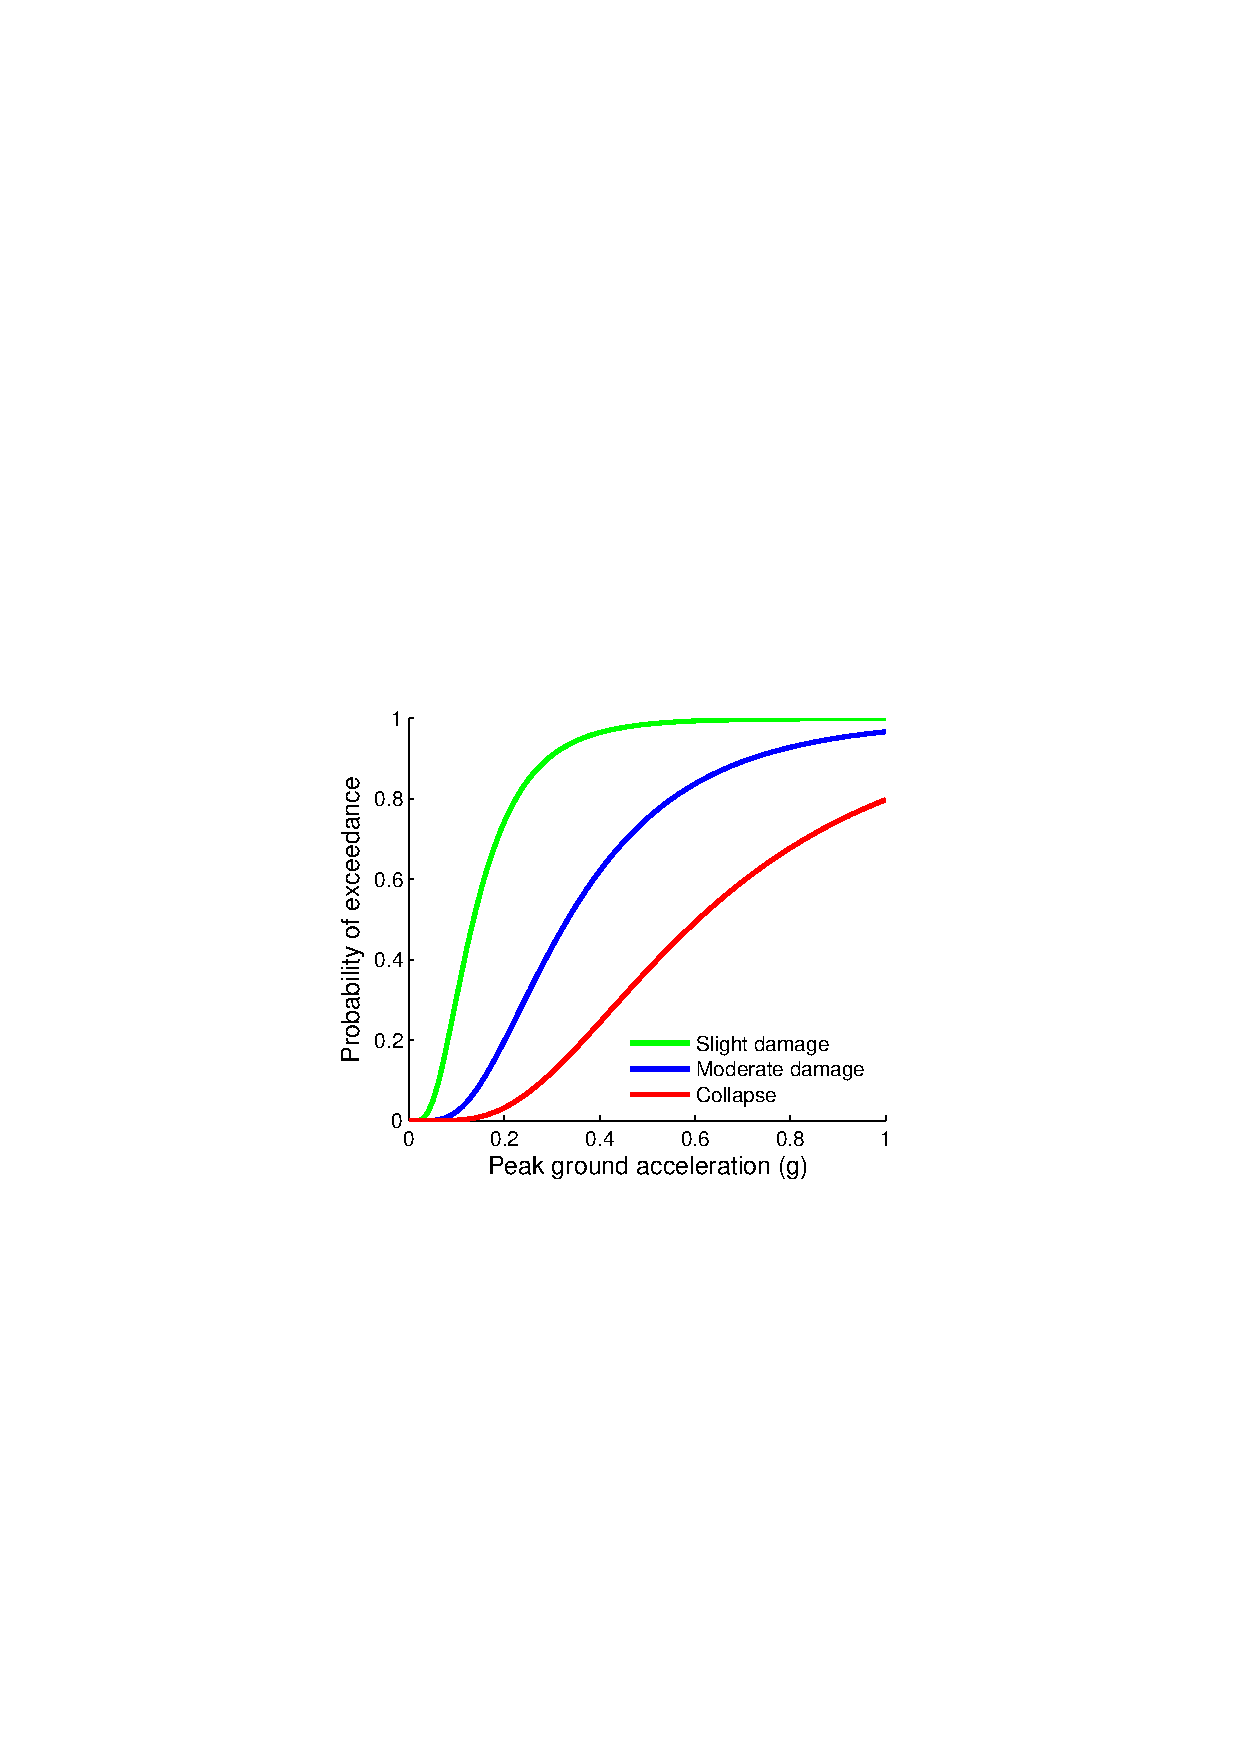
\includegraphics[width=8cm,height=6cm]{figures/risk/ConFragilityModel.pdf}
\caption{Graphical representation of a continuous fragility model.}
\label{fig:fragModelContinuous}
\end{figure}

The NRML schema to store these functions has an initial structure similar to that described for the discrete \glspl{fragility model}. Then, the continuous limit state curves are stored as illustrated below:

\begin{Verbatim}[frame=single, commandchars=\\\{\}, samepage=true]
    ...
    <\textcolor{green}{ffs noDamageLimit= 0.05}>
        <\textcolor{blue}{taxonomy} RC <\textcolor{blue}{/taxonomy}>
        <\textcolor{blue}{IML} IMT="PGA" minIML="0.0" maxIML="1.0" imlUnit="g" ><\textcolor{blue}{/IML}>
        <\textcolor{blue}{ffd} ls="slight">
            <params \textcolor{magenta}{mean}="0.16" \textcolor{magenta}{stddev}="0.11" />
        <\textcolor{blue}{/ffd}
        <\textcolor{blue}{ffd} ls="moderate">
            <params \textcolor{magenta}{mean}="0.40" \textcolor{magenta}{stddev}="0.26" />
        <\textcolor{blue}{/ffd}
        <\textcolor{blue}{ffd} ls="collapse">
            <params \textcolor{magenta}{mean}="0.73" \textcolor{magenta}{stddev}="0.48" />
        <\textcolor{blue}{/ffd}
    <\textcolor{green}{/ffs}>
<\textcolor{red}{/fragilityModel}>
</nrml>
\end{Verbatim}

Again, the set of limit state curves for each building typology needs to be stored within the field \Verb+ffs+ (fragility function set), through the definition of the following attributes:

\begin{itemize}
\item  \Verb+noDamageLimit+: this attribute defines the intensity measure level below which the probability of exceedance for all curves is zero;
\item  \Verb+type+: this parameter defines the type of probabilistic distribution being used to define the limit state curves. Currently the engine only supports lognormal distributions, however, the capability of considering other types of distributions (e.g. normal, exponential) will be developed in the future;
\item  \Verb+taxonomy+: a unique key that is used to relate each \gls{fragility function} with the relevant \glspl{asset} in the \gls{exposure model};
\item  \Verb+IML+: in this field, the intensity measure type (\Verb+IMT+) and associated units (\Verb+imlUnit+) for the limit state curves is defined, along with the minimum (\Verb+minIML+) and maximum (\Verb+maxIML+) intensity measure levels enclosing the range of applicability of the set of fragility functions;
\item  \Verb+ffc+: this field (fragility function continuous) is used to define the mean (\Verb+mean+) and standard deviation (\Verb+stddev+) of the cumulative lognormal function. In addition, the limit state for the curve being defined needs to be specified in the attribute \Verb+ls+.
\end{itemize}

\section{Consequence models}
\label{sec:consequence}
\input{oqum/risk/00c_consequence}

\section{Vulnerability models}
\label{sec:vulnerability}
In this section, the NRML schema for the \gls{vulnerability model} is
described in detail. In order to do so, a graphical representation of a
\gls{vulnerability model} (mean loss ratio for a set of intensity measure
levels) is illustrated in Figure~\ref{fig:vulModel}. Note that although the
uncertainty for each loss ratio is not represented in the aforementioned
figure, it can be considered in the input NRML file, by means of a coefficient
of variation per loss ratio and a probabilistic distribution, which can
currently be set to lognormal (LN) or Beta (BT).

\begin{figure}[ht]
\centering
\includegraphics[width=10cm,height=6cm]{figures/risk/vulnerabilityModel.pdf}
\caption{Graphical representation of a vulnerability model.}
\label{fig:vulModel}
\end{figure}

An example vulnerability model comprising three vulnerability functions is
shown below. This vulnerability model contains one function that uses the 
lognormal distribution to represent the uncertainty in the loss ratio at 
different intensity levels, one function that uses the Beta distribution, and
one function that is defined using a discrete probability mass distribution.

\inputminted[firstline=1,firstnumber=1,fontsize=\footnotesize,frame=single,linenos,bgcolor=lightgray]{xml}{oqum/risk/Verbatim/input_vulnerability.xml}\\


The initial portion of the schema contains general information that describes
some general aspects of the vulnerability model. The information in this
metadata section is common to all of the functions in the vulnerability model
and needs to be included at the beginning of every vulnerability model file.
The parameters are described below:

\begin{itemize}

    \item \Verb+id+: a unique key used to identify the \gls{vulnerability model}

    \item \Verb+assetCategory+: an optional string used to specify the type of
    \glspl{asset} for which vulnerability functions will be defined in this file 
    (e.g: buildings, lifelines)

    \item \Verb+lossCategory+: valid strings for this attribute are 
    ``structural'', ``nonstructural'', ``contents'',  
    ``business\_interruption'', and ``occupants''

    \item \Verb+description+: a brief string with further information about the
    \gls{vulnerability model}, for example, which building typologies are 
    covered or the source of the functions in the \gls{vulnerability model}

\end{itemize}

\inputminted[firstline=4,firstnumber=4,lastline=8,fontsize=\footnotesize,frame=single,linenos,bgcolor=lightgray]{xml}{oqum/risk/Verbatim/input_vulnerability.xml}\\


In order to perform probabilistic or scenario risk calculations, it is
necessary to define a vulnerability function for each building typology
present in the exposure model. The vulnerability functions require the user to
specify the distribution of the loss ratio for a set of intensity levels. The
loss ratio distributions can be defined using either a discrete or a
continuous format, and the fragility model file can include a mix of both
types of vulnerability functions. It is also possible to define a
vulnerability function using a set of deterministic loss ratios corresponding
to a set of intensity levels (i.e., ignoring the uncertainty in the
conditional loss ratios).

The following snippet from the above vulnerability model example file defines
a vulnerability function modelling the uncertainty in the conditional loss
ratios using a (continuous) lognormal distribution:

\inputminted[firstline=10,firstnumber=10,lastline=14,fontsize=\footnotesize,frame=single,linenos,bgcolor=lightgray]{xml}{oqum/risk/Verbatim/input_vulnerability.xml}\\

The following attributes are needed to define a vulnerability function which
uses a continuous distribution to model the uncertainty in the conditional
loss ratios:

\begin{itemize}

    \item \Verb+id+: a unique key used to identify the \gls{taxonomy} for 
    which the function is being defined. This key is used to relate the 
    \gls{vulnerability function} with the relevant \gls{asset} in the 
    \gls{exposure model}.

    \item \Verb+dist+: for vulnerability function which use a continuous 
    distribution to model the uncertainty in the conditional loss ratios, 
    this attribute should be set to either ``\Verb+LN+'' if using the lognormal
    distribution, or to ``\Verb+BT+'' if using the Beta distribution.

    \item \Verb+imls+: this attribute specifies the list of intensity levels
    for which the parameters of the conditional loss ratio distributions will
    be defined. In addition, it is also necessary to define the intensity 
    measure type (\Verb+imt+).

    \item \Verb+meanLRs+: this field is used to define the mean loss ratios
    for this \gls{vulnerability function} for each of the intensity levels
    defined by the attribute \Verb+imls+. The number of mean loss ratios
    defined by the \Verb+meanLRs+ attribute must be equal to the number of
    intensity levels defined by the attribute \Verb+imls+.

    \item \Verb+covLRs+: this field is used to define the coefficient of 
    variation for the conditional distribution of the loss ratios for this
    \gls{vulnerability function} for each of the intensity levels defined by
    the attribute \Verb+imls+. The number of coefficients of variation of loss
    ratios defined by the \Verb+covLRs+ attribute must be equal to the number
    of intensity levels defined by the attribute \Verb+imls+. The uncertainty
    in the conditional loss ratios can be ignored by setting all of the
    \Verb+covLRs+ for a given \gls{vulnerability function} to zero.

\end{itemize}

Several methodologies to derive vulnerability functions are currently being
evaluated by \gls{acr:gem} and have been included as part of the Risk
Modeller's Toolkit, the code for which can be found on a public repository at
GitHub at the following address
\href{http://github.com/gemsciencetools/rmtk}{http://github.com/gemsciencetools/rmtk}.

Scripts to convert \glspl{vulnerability function} in CSV format or as Excel or
ASCII files into NRML are also under development, and can be found at the
OpenQuake platform at the following address:
\href{https://platform.openquake.org/risk_input_preparation_toolkit/}{https://platform.openquake.org/risk\_input\_preparation\_toolkit/}.


\section{Calculation workflows}
\label{sec:risk_workflows}
\subsection{Scenario Damage Assessment}
\index{OpenQuake-engine!Risk calculation workflows!Scenario Damage Assessment}
\label{subsec:workflow_scenario_damage}
This calculator is capable of assessing the damage distribution due to a
single scenario earthquake, for a collection of assets. Similarly to the
previous calculator, in order to perform the necessary risk calculations one
or a set of ground motion fields are required, which can be derived using the
oq-hazardlib, or introduced in the OpenQuake-engine using the appropriate NRML
schema. In this calculator, a fragility model is combined with the
distribution of ground motion at the location of each asset, to estimate the
number or area of buildings in each damage state. The damage distribution can
be extracted per asset, per building typology (taxonomy) or considering all of
the assets simultaneously (total damage distribution). In addition, this
calculator also provides collapse maps, which contain the spatial distribution
of the number or area of collapsed buildings throughout the region of
interest. The input/output structure for this calculator is presented in
Figure~\ref{fig:io-structure-scenario-damage}.

\begin{figure}[ht]
\centering
\includegraphics[width=9cm,height=7cm]{figures/risk/io-structure-scenario-damage.pdf}
\caption{Scenario Damage Calculator input/output structure.}
\label{fig:io-structure-scenario-damage}
\end{figure}

\subsection{Scenario Risk Assessment}
\index{OpenQuake-engine!Risk calculation workflows!Scenario Risk Assessment}
\label{subsec:workflow_scenario_risk}
This calculator computes loss maps and loss statistics due to a single seismic
event, for a collection of assets. The hazard input can be a single ground
motion field (e.g. the median distribution of ground motion in the region of
interest) or a set of ground motion fields allowing the characterisation of
the inter- and intra-event variability from the GMPE. It is noted that the
hazard input can either be calculated using the hazard component of OpenQuake-
engine (oq-hazardlib), or provided to the risk component iian external file
following the respective Natural hazards' Risk Markup Language (NRML) schema
(see \href{http://github.com/gem/oq-nrmllib}{oq-nrmllib}). A vulnerability
model is combined with the distribution of the ground motions at each asset
location to calculate the loss distribution for each asset, as well as the
statistics of the total loss throughout the region of interest. The required
input files and resulting output files are depicted in
Figure~\ref{fig:io-structure-scenario-risk}.

\begin{figure}[ht]
\centering
\includegraphics[width=9cm,height=7cm]{figures/risk/io-structure-scenario-risk.pdf}
\caption{Scenario Risk Calculator input/output structure.}
\label{fig:io-structure-scenario-risk}
\end{figure}

\subsection{Classical Probabilistic Seismic Damage Analysis}
\index{OpenQuake-engine!Risk calculation workflows!Classical Probabilistic Seismic Damage Analysis}
\label{subsec:workflow_classical_damage}
The classical PSHA-based damage calculator convolves through numerical integration, the damage state fragility functions for an asset with the seismic hazard curve at the location of the asset. The main results of this calculator are damage distribution statistics for each asset, which describe the expected fraction of buildings in each damage state. Furthermore, a probabilistic collapse map can be extracted giving the probability of collapse for each asset within the specified time period. Damage distribution aggregated by taxonomy or of the total portfolio (considering all assets in the exposure model) can not be extracted using this calculator, as the spatial correlation of the ground motion residuals is not taken into consideration. The input and output files involved in this calculator are presented in Figure~\ref{fig:ClassicalDamage}.

\begin{figure}[ht]
\centering
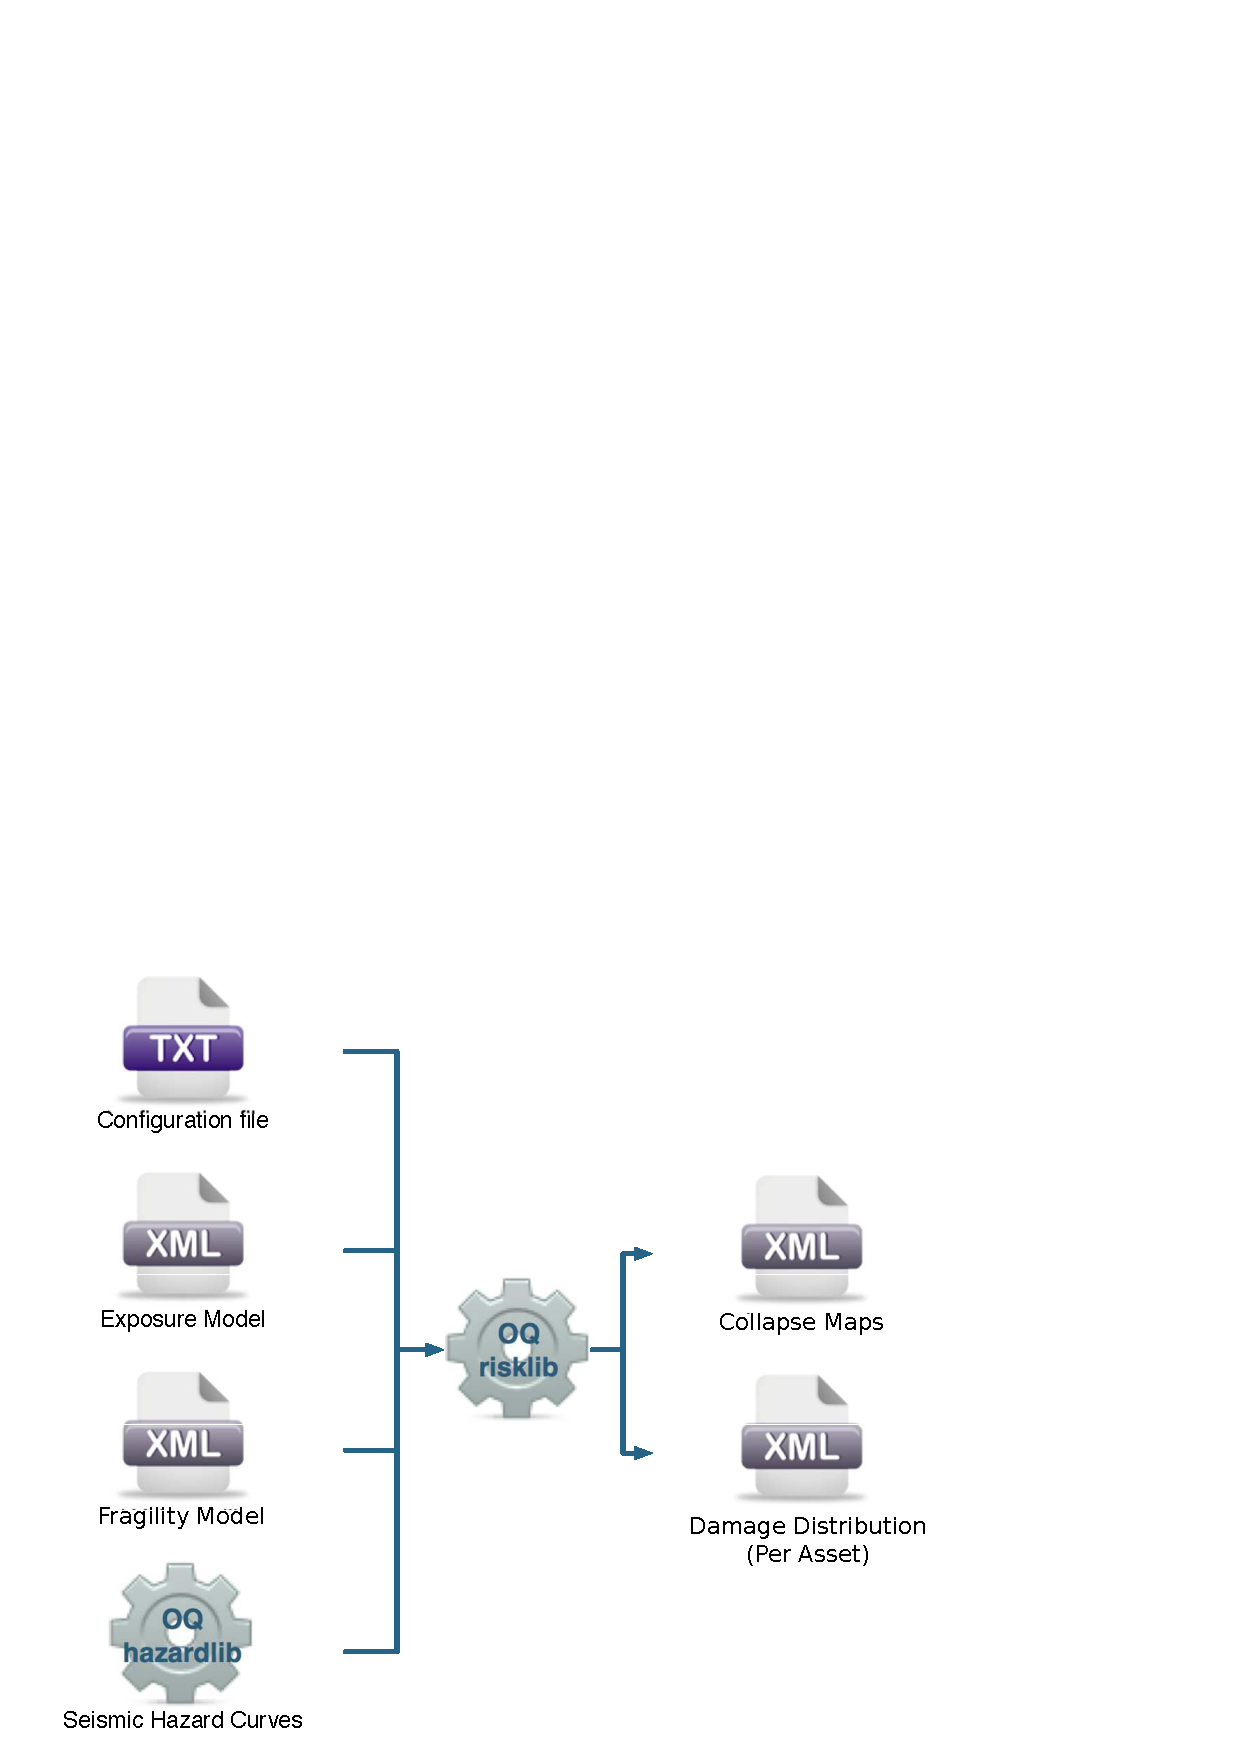
\includegraphics[width=9cm,height=7cm]{figures/risk/ClassicalDamage.pdf}
\caption{Classical PSHA-based Damage Calculator input/output structure.}
\label{fig:ClassicalDamage}
\end{figure}

\subsection{Classical Probabilistic Seismic Risk Analysis}
\index{OpenQuake-engine!Risk calculation workflows!Classical Probabilistic Seismic Risk Analysis}
\label{subsec:workflow_classical_risk}
In this calculator, probabilistic seismic hazard is employed to calculate a loss exceedance curve for each asset, through the usage of seismic hazard curves. A convolution between the vulnerability function and the hazard curve at location of the asset is performed, leading to the probability of exceeding a set of loss ratios. Each loss ratio is multiplied by the asset value to obtain the final loss exceedance curve. Furthermore, probabilistic loss maps can be extracted by interpolating the loss curves at each location by various probabilities of exceedance. Unlike what was described in the previous calculator, a total loss curve (considering all assets in the exposure model) can not be extracted using this calculator, as the correlation of the ground motion residuals and vulnerability uncertainty is not taken into consideration. The input and output files involved in this calculator are presented in Figure~\ref{fig:ClassicalRisk}.

\begin{figure}[ht]
\centering
\includegraphics[width=9cm,height=7cm]{figures/risk/ClassicalRisk.pdf}
\caption{Classical PSHA-based Risk Calculator input/output structure.}
\label{fig:ClassicalRisk}
\end{figure}

\subsection{Event-Based Probabilistic Seismic Risk Analysis}
\index{OpenQuake-engine!Risk calculation workflows!Event-Based Probabilistic Seismic Risk Analysis}
\label{subsec:workflow_event_based_risk}
In this calculator, loss exceedance curves and loss maps for various return
periods can be calculated, based on probabilistic seismic hazard, with an
event-based approach. A large number of stochastic event sets are generated,
and the associated ground motion fields for each event are used together with
a vulnerability model to compute the individual (per asset) and total (sum of
all the losses per event) losses. Then, this distribution of losses is
employed to derive a loss exceedance curve per asset, as well as a total loss
exceedance curve representative of the complete building portfolio.
Furthermore, oq-risklib can also compute loss maps for various return periods
by interpolating each individual loss curve with the respective probability of
exceedance. In Figure~\ref{fig:io-structure-event-based-risk}, the
input/output scheme of this calculator is illustrated.

\begin{figure}[ht]
\centering
\includegraphics[width=9cm,height=7cm]{figures/risk/io-structure-event-based-risk.pdf}
\caption{Probabilistic Event-based Risk Calculator input/output structure.}
\label{fig:io-structure-event-based-risk}
\end{figure}

\subsection{Retrofit Benefit-Cost Ratio Analysis}
\index{OpenQuake-engine!Risk calculation workflows!Retrofit Benefit-Cost Ratio Analysis}
\label{subsec:workflow_benefit_cost}
\input{oqum/risk/00e_workflow_benefit_cost}

\cleardoublepage